\cleardoublepage

\chapter{EEG and event-related potentials}
\label{sec:eeg}

\section{Electro-encephalography (EEG)}
\label{sec:eeg:eeg}

The first recording of the electric field of the human brain was made by the German psychiatrist Hans Berger in 1924. He named this recording electroencephalogram (EEG; \citealp{berger_uber_1929}). Since then, EEG and event-related potentials (ERP; see next section) have become one of the most prominent technique in research (e.g. neuroscience, psychology) and medical settings (e.g. epilepsy, sleep disorders). EEG records voltage fluctuations resulting from ionic current within large assemblies of neurons in the brain. The brain electrical activity is measured with electrodes that are placed either along the scalp or, in rarer circumstances, directly on the exposed surface of the brain (electro-corticography or intra-cranial EEG). Through the current thesis, we will focus solely on the former and non-invasive, scalp EEG method, which is also one of the three essential electrophysiological measurements of polysomnography, along with EOG and EMG (see section \ref{sec:dream-research:sleep:stages}).

\subsection{International 10-20 system}
\label{sec:eeg:eeg:10-20}

EEG is generally recorded from multiple electrodes distributed across the scalp. To allow reproducibility both within and between individuals, the placement of these electrodes is defined in the internationally standardized 10-20 system, which relies on the relationship between the location of an electrode and the underlying area of cerebral cortex (Figure \ref{fig:methods:10-20}). Electrode location are determined using two standard anatomical landmarks, the nasion and inion, respectively located between the eyes and at the back of the skull. From these points, the skull perimeters are measured in the transverse and median planes and electrode locations are determined by dividing these perimeters into 10\% and 20\% distance intervals. Electrodes names refer to their locations on the cerebral cortex. Thus, the first letter refers to the brain lobe on which they are located (F = frontal, C = central, P = parietal, O = occipital), while the number corresponds to the hemispheres (3 = left, 4 = right). For example, F3 is located on the left hemisphere of the frontal lobe, while P4 lies on the right hemisphere of the parietal lobe.

\begin{figure}[htb]
	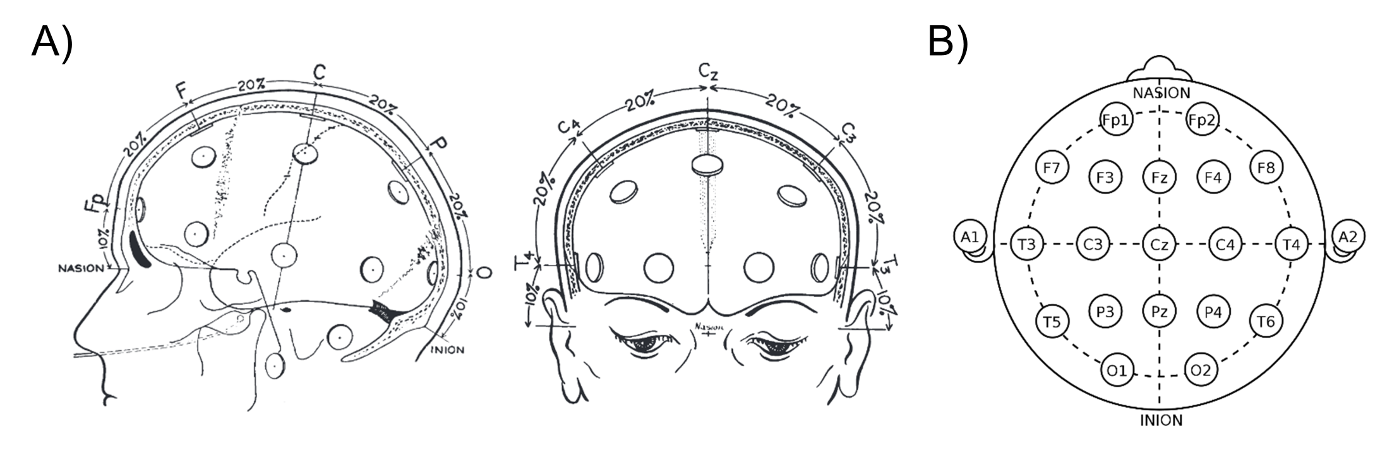
\includegraphics[width=\textwidth]{Fig/Methods/EEG_10-20/EEG_10-20.png}
	\caption[Electrode locations of International 10-20 system for EEG recording]{Electrode locations of International 10-20 system for EEG recording. A) Lateral and frontal views of the skull showing the methods of measurement for electrode placement (adapted from \citealp{klem_ten-twenty_1999}). B) Single plane projection of the head showing all standard positions and names of electrodes according to the 10-20 system. }
	\label{fig:methods:10-20}
\end{figure}

\subsection{Amplification, filtering and montage}
\label{sec:eeg:eeg:ampli}

The brain electrical activity is quite small (usually under 100 µV). For that reason, the EEG signal recorded on the scalp must be first amplified by several thousand times. In modern, digital EEG, the signal from each channel is then turned into a series of discrete digital values, with a sampling frequency generally comprised between 200 to 5000 Hz. The signal is then filtered and displayed on a computer screen using dedicated softwares such as Elan \citep{aguera_elan:_2011} or EEGLAB \citep{delorme_eeglab:_2004}. Typical filters include high-pass (<0.1 Hz), low-pass (35-70 Hz), and notch (50 or 60 Hz) to remove very slow artefacts, high-frequency artefacts (such as electromyographic activity) and electrical noise, respectively.
Since the EEG is measured as the voltage (i.e. potential for electrical charges to move between two locations) between two electrodes, the display of EEG may be set up in several ways, referred to as montage. In the standard, referential montage, a single reference electrode, located at a site thought to be electrically neutral, such as the earlobe or the mastoid, is typically used for all the active scalp electrodes. By contrast, in the average reference montage, the averaged signal across all electrodes is used as the common reference for each channel.

\subsection{Neural oscillations}
\label{sec:eeg:eeg:neural}

The spontaneous brain electrical activity is characterized by rhythmic oscillations, which are sometimes referred to as neural oscillations or, more popularly, as \q{brain waves}. These oscillations are generated by the summation of synchronous activity of thousands or millions or neurons (mainly cortical pyramidal neurons). They have characteristic frequency ranges, spatial distributions and are associated with different states of brain functioning (e.g. waking and the various sleep stages; see Figure \ref{fig:methods:neural}).

\begin{figure}[htb]
	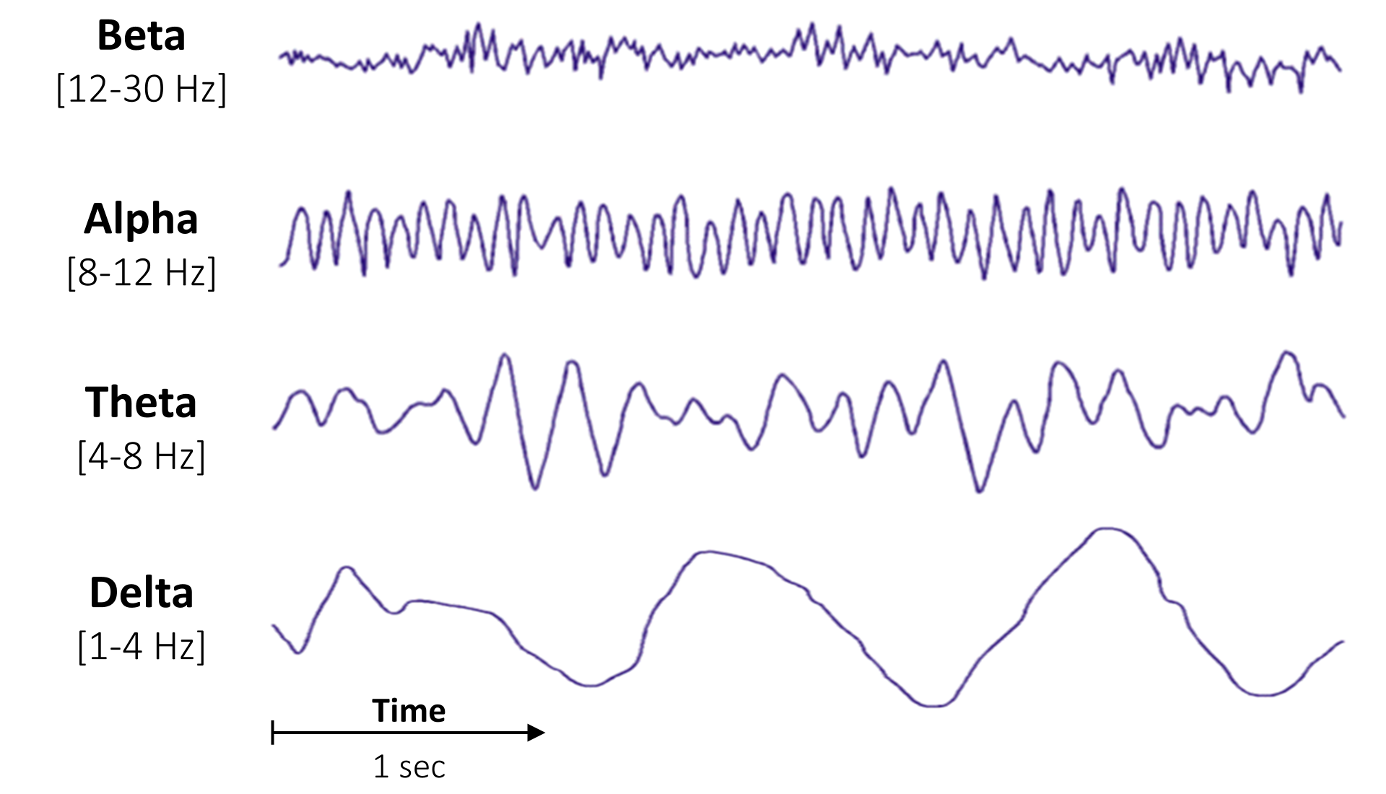
\includegraphics[width=\textwidth]{Fig/Methods/EEG_BrainWaves/EEG_Brain_Waves.png}
	\caption[Brain rhythms]{Brain rhythms. Beta waves are prominent over occipital and parietal areas during normal waking wakefulness. Alpha waves are prominent in occipital regions during eyes-closed wakefulness. Theta waves are detectable during N2 sleep and REM sleep. Delta waves are visible during N3 sleep (also called slow-wave sleep or deep sleep) and have a large amplitude (>75 µV) due to a high level of neural synchronization.}
	\label{fig:methods:neural}
\end{figure}

\section{Event-related potentials (ERP)}
\label{sec:eeg:erp}

\subsection{Definition and methods}
\label{sec:eeg:erp:def}

Event-related potentials (ERPs) are \q{electrical potentials generated by the brain that are related to specific internal or external events such as stimuli, responses or decisions} \citep{luck_introduction_2014}. A single ERP, usually recorded by means of scalp EEG, has an amplitude ranging from 0.5 to 15 µV, and is therefore much lower than the spontaneous background EEG (100 µV). As a consequence, a single ERP is not visible to the naked eye in the EEG signal. In order to disentangle and reveal the specific relevant ERP from the irrelevant background EEG, ERP technique relies on the mathematical principle of summation. It consists of averaging hundreds of time-locked repetitions of the same experimental condition in order to attenuate activities that are unrelated to the specific internal or external event.
The resulting waveform contains a series of positive and negative peaks (components) that are thought to reflect activity (i.e. postsynaptic potentials) in underlying generators within the brain. These components are usually referred to with acronyms (e.g. contingent negative variation, CNV) or by a letter indicating polarity (N = negative, P = positive), followed by a number indicating the latency in milliseconds from stimulus onset (e.g. N100 is a negative peak arising approximatively 100 ms after stimulus). Early components, which arise approximatively less than 80 ms after the stimulus, are thought to reflect sensory processes and are therefore intrinsically linked to the physical characteristics of the stimulus. By contrast, late components (>100ms) are thought to reflect more cognitive processes such as attention, memory and response preparation. They differ from the former in the sense that they are not systematically elicited but rather require the participant to be involved in some stimulus-related task (e.g. a detection task). While some potentials are easily obtain by repetition of stimuli (e.g. the N100 potential, elicited by perception of auditory stimuli), others potentials are elicited by more complex paradigm. One of the most famous is probably the oddball-paradigm, in which low-probability target (or \textit{deviant}) items are mixed with high-probability non-target (or \textit{standard}) items. Target items elicit a late positive component, the P300, though to reflect brain processes involved in stimulus evaluation or categorization.

\begin{figure}[htb]
	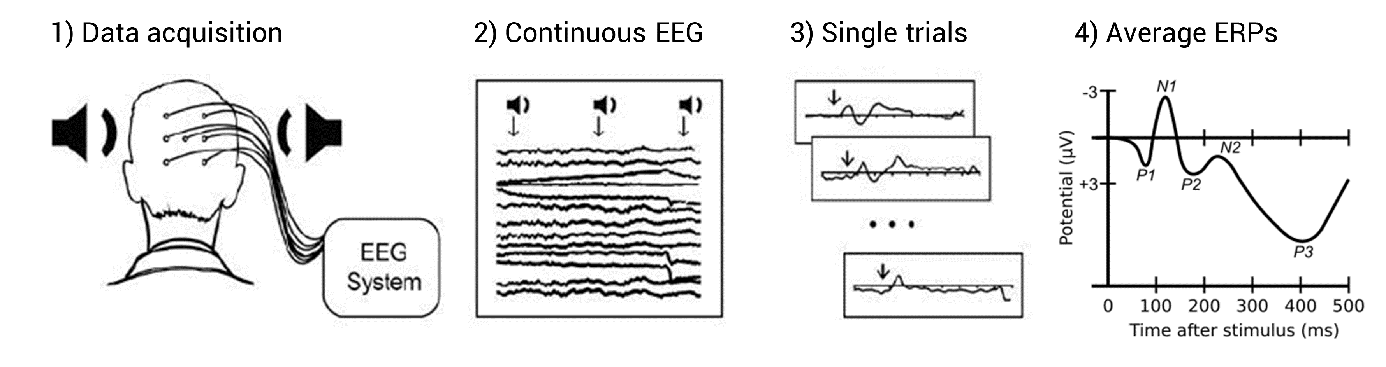
\includegraphics[width=\textwidth]{Fig/Methods/ERP/ERP.png}
	\caption[Schematic representation of ERP acquisition]{Schematic representation of ERP acquisition. (1) Scalp electrodes record electrical brain activity while auditory stimuli are presented repeatedly through headphones or speakers. (2) Stimulus onset/offset markers are recorded along with the continuous EEG signal. (3) Individual segments locked to stimulus onset are extracted from the continuous EEG and include a brief pre-stimulus baseline in addition to post-stimulus period of interest. (D) Averaged ERP waveform showing several components (including the N100 and P300) reflecting time- and phase-locked neural activity associated with stimulus processing. Note that the ERP is plotted with negative voltages upward, a common, but not universal, practice in ERP research. Adapted from \citet{key_human_2016}}
	\label{fig:methods:erp}
\end{figure}

\subsection{The use of ERP in sleep research}
\label{sec:eeg:erp:erp}

ERP is a method of choice for the investigation of the normal and pathological human sleep \citep{bastuji_evoked_1999, colrain_use_2007}. One reason for this is that it allows to study objectively information processing during sleep, limited otherwise by the lack of the ability of subjects to make verbal or motor responses to stimuli. It provides a powerful, objective and non-invasive means to study for example the extent of sensory integration during sleep, or the neurological abnormalities related to sleep disorders, or sleep inertia upon waking \citep{bastuji_event-related_2003}.
ERP studies greatly improved our understanding of sleep, from the classical view that sleep is a “little death” (illustrated by the fraternal link between Hypnos, God of Sleep, and Thanatos, God of Death, in the Greek mythology; see \citealp{mazza_asleep_2014}), to the emerging idea that sleep is a dynamic process in which complex cognitive processing occur \citep{andrillon_sleeping_2016}. For example, a P300 component has been observed during REM sleep in response to target stimuli presented within an oddball paradigm \citep{bastuji_brain_1995}. Similarly, there is a persistence of the brain’s ability to detect semantic incongruity during REM sleep  (N400; \citealp{perrin_detection_2002}).
It should however be noted that considerable differences exist between waking, NREM and REM sleep ERP components \citep{bastuji_evoked_1999, colrain_use_2007}. Specifically, while early sensory components (i.e. peripheral and brainstem responses) remain unaffected by the sleep cycle, early cortical responses are drastically modified, in part because the thalamus stops relaying sensory information to the brain. Finally, late cortical responses displays profound changes during NREM sleep, which revert in REM sleep.
